\section{Aufbau}

Zwei wichtige Bauteile in diesem Experiment sind Polarisationsfilter und PBSCs:

\paragraph{Polarisationsfilter}
Mit einem Polarisationsfilter wird der Anteil des Lichtes absorbiert, dessen Polarisationsachse senkrecht zu einer einstellbaren Achse liegt. Durch eine Drehung des Polarisationsfilters kann bewirkt werden, dass nur die gewünschten Lichtanteile transmittiert werden.

\paragraph{Polarizing beam-splitter cube, PBSC}
\label{par:pbsc}
Ein PBSC ist ein Glaswürfel, der einen halbdurchlässigen Spiegel enthält, welcher zwischen zwei gegenüberliegenden Kanten verläuft. Auf diesem ist eine dünne dielektrische Schicht aufgetragen, welche bewirkt, dass einfallendes Licht in zwei Komponenten aufgeteilt wird, welche zueinander senkrecht polarisiert sind. Dabei durchquert eine Komponente das Glas, während die andere um \SI{90}{\degree} reflektiert wird.



\begin{figure}
\centering
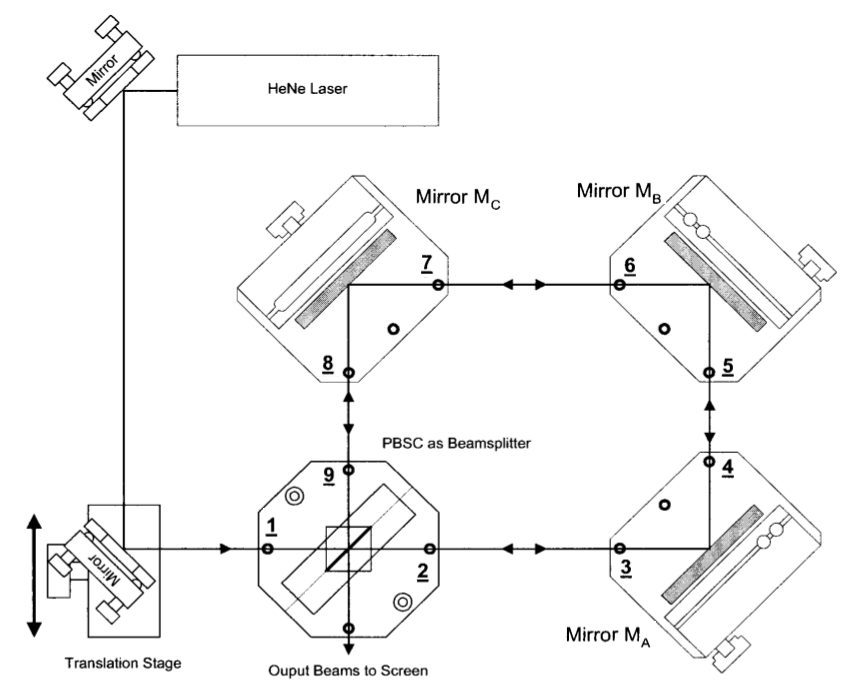
\includegraphics[width=0.7\linewidth]{img/aufbau.png}
\caption{Schematische Darstellung des verwendeten Sagnac-Interferometers. Die Beschriftungen wurden einem Bild der gleichen Quelle entnommen. \cite{V64}}
\label{fig:aufbau}
\end{figure}

\subsection{Aufbau und Besonderheiten des Sagnac-Interferometers}
Das in diesem Versuch verwendete Sagnac-Interferometer besteht im Wesentlichen aus einem Helium-Neon-Laser, welcher, laut seiner Beschriftung, linear polarisiertes Licht mit einer Wellenlänge von \SI{632.8}{\nano\metre} \cite{V64} liefert, fünf Spiegeln, einem PBSC und einem Polarisationsfilter. Desweiteren werden für spezielle Messverfahren noch ein weiterer PBSC, ein weiterer Polarisationsfilter und zwei Photodioden verwendet, sowie zur Untersuchung der Brechungsindizes zwei im festen Winkel zueinander angeordnete Glasplatten und eine Gaskammer. Eine schematische Zeichnung des Interferometers ist in Abbildung \ref{fig:aufbau} zu sehen.

Alle Bauteile werden an einem Schraubbrett befestigt und während der Messungen von einem Plexiglaskäfig überdacht, um Luftströmung innerhalb der Interferometeranordnung zu verhindern, die messbare Störungen verusachen würden. Die Besonderheit dieses Interferometertyps liegt in der Toleranz gegenüber Vibrationen der Apparatur, da die gegenläufigen Strahlen die selben Weglängen zurücklegen und somit die Phasendifferenz der beiden Strahlen weitestgehend unverändert bleibt. Experimente mit einem einzelnen Strahl im Inneren des Interferometers sind möglich, wenn der eingehende Strahl mit einem horizontal verschiebbaren Spigel verschoben wird. Dadurch erhalten die aufgeteilten Strahlen horizontal einen räumlichen Abstand, wobei sich der zurückgelegte Weg der beiden Strahlen um den gleichen Wert ändert, sodass auch dadurch keine Phasendifferenz auftritt.

\subsection{Justierung der Apparatur}
Die Justierung des Sagnac Interferometers wird mittels der in Abbildung \ref{fig:aufbau} verwendeten Bezeichnung der Spiegel und Halteplätze für Justierhilfen erläutert. Die Justierhilfen
sind Metallplatten mit kleinen Löchern zum Durchlassen des Laserlichts.

Als erstes werden der HeNe-Laser und die beiden Steuerspiegel auf dem Schraubbrett befestigt und ausgerichtet. Dann wird der PBSC und die Spiegel A, B und C, wie in Abbildung \ref{fig:aufbau} zu sehen, platziert. Der durch den PBSC reflektierte Strahl wird zunächst blockiert, um Spiegel A in seine endgültige Position zu bringen. Die beiden Stuerspiegel werden so justiert, dass das Strahl in den Positionen 1, 2 und 3 zentral durch die Löcher der Justierhilfe treten kann. Anschließend wird der vom PBSC durchgelassene Strahl blockiert und Spiegel C befestigt. Dafür wird der PBSC so fixiert, dass auch hier der Lichtstrahl durch die Justierhilfe an den Positionen 9 und 8 treten kann.

Die Justierilfen werden nun in die Plätze 5 und 6 gesteckt und die Spiegel A und C so bewegt und anshcließend festgeschraubt, dass der Strahl auch hier durch die Justierhilfe tritt. Wenn das getan wurde, werden die Justierhilfen in die Positionen 4 und 7 gesteckt. Spiegel C wird zurechtgerückt, bis beide Teilstrahlen durch jeweils beide Seiten der Löcher der Justierhilfen gelangen. Spiegel C wird daraufhin auch an dem Schraubbrett festgeschraubt.

Zu diesem Zeitpunkt sind die beiden Teilstrahlen im Interferometer noch nicht räumlich getrennt. Werden die aus der vierten Seite des PBSCs austretenden Lichtstrahlen auf einem Schirm betrachtet, zeigt
sich aber, dass die beiden Lichtstrahlen sich nicht vollkommen überlappen. Um dies zu erreichen, werden die Fingerschrauben bei den Spiegeln A und C verwendet. Nach diesem Schritt sind die Spiegel
richtig justiert.

Wird vor den PBSC ein Polarisationsfilter gestellt, können die Intensitäten der beiden Teilstrahlen im Interferometer eingestellt werden. Wird der zweite Steuerspiegel seitlich bewegt kann eine räumliche Trennung der vom PBSC getrennten Strahlen erreicht werden. Um die Qualität des (noch nicht interferierenden) Strahls, der aus der vierten Seite des PBSC tritt, zu verbessern und die beiden enstehenden Strahlen aufeinander auszurichten, kann noch an den Fingerschrauben der Spiegel A, B und C gedreht werden.
